\documentclass[xcolor=dvipsnames,hyperref={breaklinks=true},mathserif,professionalfont,dvipdfmx,12pt]{beamer}
\usepackage[ipaex]{pxchfon}
\usepackage{amsmath,amssymb}
\usepackage{amsthm}
\usepackage{ascmac}

\usepackage[utf8]{inputenc}
\usepackage{bm}
\usepackage{here}
\usepackage{enumerate}
\usepackage{bxdpx-beamer} %dvipdfmc対応
\usepackage{pxjahyper} %しおりの和文対応
\usepackage{minijs} %jsarticleのミニ版
\usepackage{otf}
\usepackage{helvet}
\usepackage{breqn}
\usepackage{color}
\usepackage{xcolor}
\usepackage{graphicx}

\usepackage[style=chem-angew,backend=bibtex]{biblatex}
\AtEveryCitekey{\iffootnote{\tiny}{}}
\usepackage{filecontents}
\addbibresource{Reference.bib}


%hyperlink等
\usepackage{hyperref}
\usepackage{pxjahyper}

\renewcommand{\kanjifamilydefault}{\gtdefault}
%TikZ
\usepackage{tikz}
\usetikzlibrary{positioning}
\usetikzlibrary{arrows.meta}
\usetikzlibrary{bending}
\usetikzlibrary{shapes.geometric}
\usetikzlibrary {shapes.misc}

\usepackage[T1]{fontenc}
\usepackage{lmodern}
\usepackage{gnuplot-lua-tikz}
\usepackage{gnuplottex}

\usepackage[absolute,overlay]{textpos}
% \usepackage[colorgrid,gridunit=pt,texcoord]{eso-pic}%グリッド表示


\renewcommand{\figurename}{図}
\renewcommand{\tablename}{表}


\setbeamertemplate{caption}[numbered]

\title{Physics Informed Neural Networks (PINNs)}
\subtitle{物理法則に基づいた機械学習手法}
\author{YokoPhys-h}
\date{\today}
\institute{hoge大学大学院}
\titlegraphic{
\includegraphics[scale=0.3]{icon_YokoPhys.png}}




% \usetheme{Madrid}
\usetheme{Montpellier}
% \usetheme{AnnArbor}
%\usetheme{Copenhagen}
% \usecolortheme[RGB={0, 126, 15}]{structure}

% \usetheme{Rochester}

\usecolortheme[named=MidnightBlue]{structure} % 色指定
\usefonttheme{professionalfonts}

\setbeamertemplate{blocks}[rounded][shadow=true]
%itemizeの記号設定
\setbeamertemplate{itemize item}[ball] 
\setbeamertemplate{itemize subitem}[triangle]
\setbeamertemplate{itemize subsubitem}[circle]

% \setbeamertemplate{navigation symbols}{}%ナビゲーションシンボル消去
\setbeamertemplate{footline}[page number] %ページ番号
%\setbeamertemplate{navigation symbols}[horizontal]

\makeatletter
\def\pgfutil@insertatbegincurrentpagefrombox#1{%
  \edef\pgf@temp{\the\wd\pgfutil@abb}%
  \global\setbox\pgfutil@abb\hbox{%
    \unhbox\pgfutil@abb%
    \hskip\dimexpr2in-2\hoffset-\pgf@temp\relax% changed
    #1%
    \hskip\dimexpr-2in-2\hoffset\relax% new
  }%
}
\makeatother


\begin{document}

\begin{frame}[plain]
  \titlepage
\end{frame}
\begin{frame}
  \frametitle{Contents}
  \tableofcontents
\end{frame}

\section{研究背景}

\begin{frame}
  \frametitle{研究背景}
  例: 自由落下運動\cite{_HuaTinoNVIDIASimNetDemoShiwareteiruPhysicsInformed_}

  運動方程式
  \begin{align*}
    m\dfrac{\mathrm{d}^2 x(t)}{\mathrm{d}t^2}=mg
  \end{align*}
  \vspace{-22pt}
  \begin{enumerate}
    \item 代数的解法\\
    微分方程式を解析的に解く. 
    \begin{align*}
      \dfrac{\mathrm{d}x(t)}{\mathrm{d}t}=v(t)=gt+v_0\\
      \alert{x_0=\dfrac{1}{2}gt^2+v_0t+x_0}
    \end{align*}
    非線形微分方程式など陽に解けない微分方程式がある.
  \end{enumerate}
\end{frame} 

\begin{frame}
  % \frametitle{研究背景}
  \begin{enumerate}
  \setcounter{enumi}{1}
    \item シミュレーション的解法\\
    微分方程式をEuler法, Runge-Kutta法などを用いて数値的に解く. 
    \begin{align*}
      m\dfrac{\mathrm{d}^2 x(t)}{\mathrm{d}t^2}=mg\quad 
       \Rightarrow\quad &x(t+1)=x(t)=\Delta \dfrac{\mathrm{d}x(t)}{\mathrm{d}t}\\
      &\dfrac{\mathrm{d}x(t+1)}{\mathrm{d}t}=\dfrac{\mathrm{d}x(t)}{\mathrm{d}t}+\Delta g
    \end{align*}
    数値解
    \begin{align*}
      \begin{aligned}
        &t=0\quad x(0)=0\\
      &t=1\quad x(1)=4.9\\
      &t=2\quad x(2)=19.6\\
      &\ \ \ \ \vdots\quad\ \ \ \ \ \ \ \ \ \ \  \vdots
      \end{aligned}
    \end{align*}
    初期条件から順に計算する必要があり, 任意の時刻における変数値を求めることができない. 
  \end{enumerate}
\end{frame}

\begin{frame}
  % \frametitle{研究背景}
  \begin{enumerate}
    \setcounter{enumi}{2}
    \item データ駆動アプローチ的解法\\
    シミュレーションで求めた数値解を基に損失関数を定義し, 入出力の関係をNeural Networksで近似する.\\
    \vspace{3pt}
    数値解
      \begin{flalign*}
        &t=0\quad x(0)=0&\\
      &t=1\quad x(1)=4.9&\\
      &t=2\quad x(2)=19.6&\\
      &\ \ \ \ \vdots\quad\ \ \ \ \ \ \ \ \ \ \  \vdots&
    \end{flalign*}
    \begin{textblock*}{0.4\linewidth}(200pt, 90pt)
    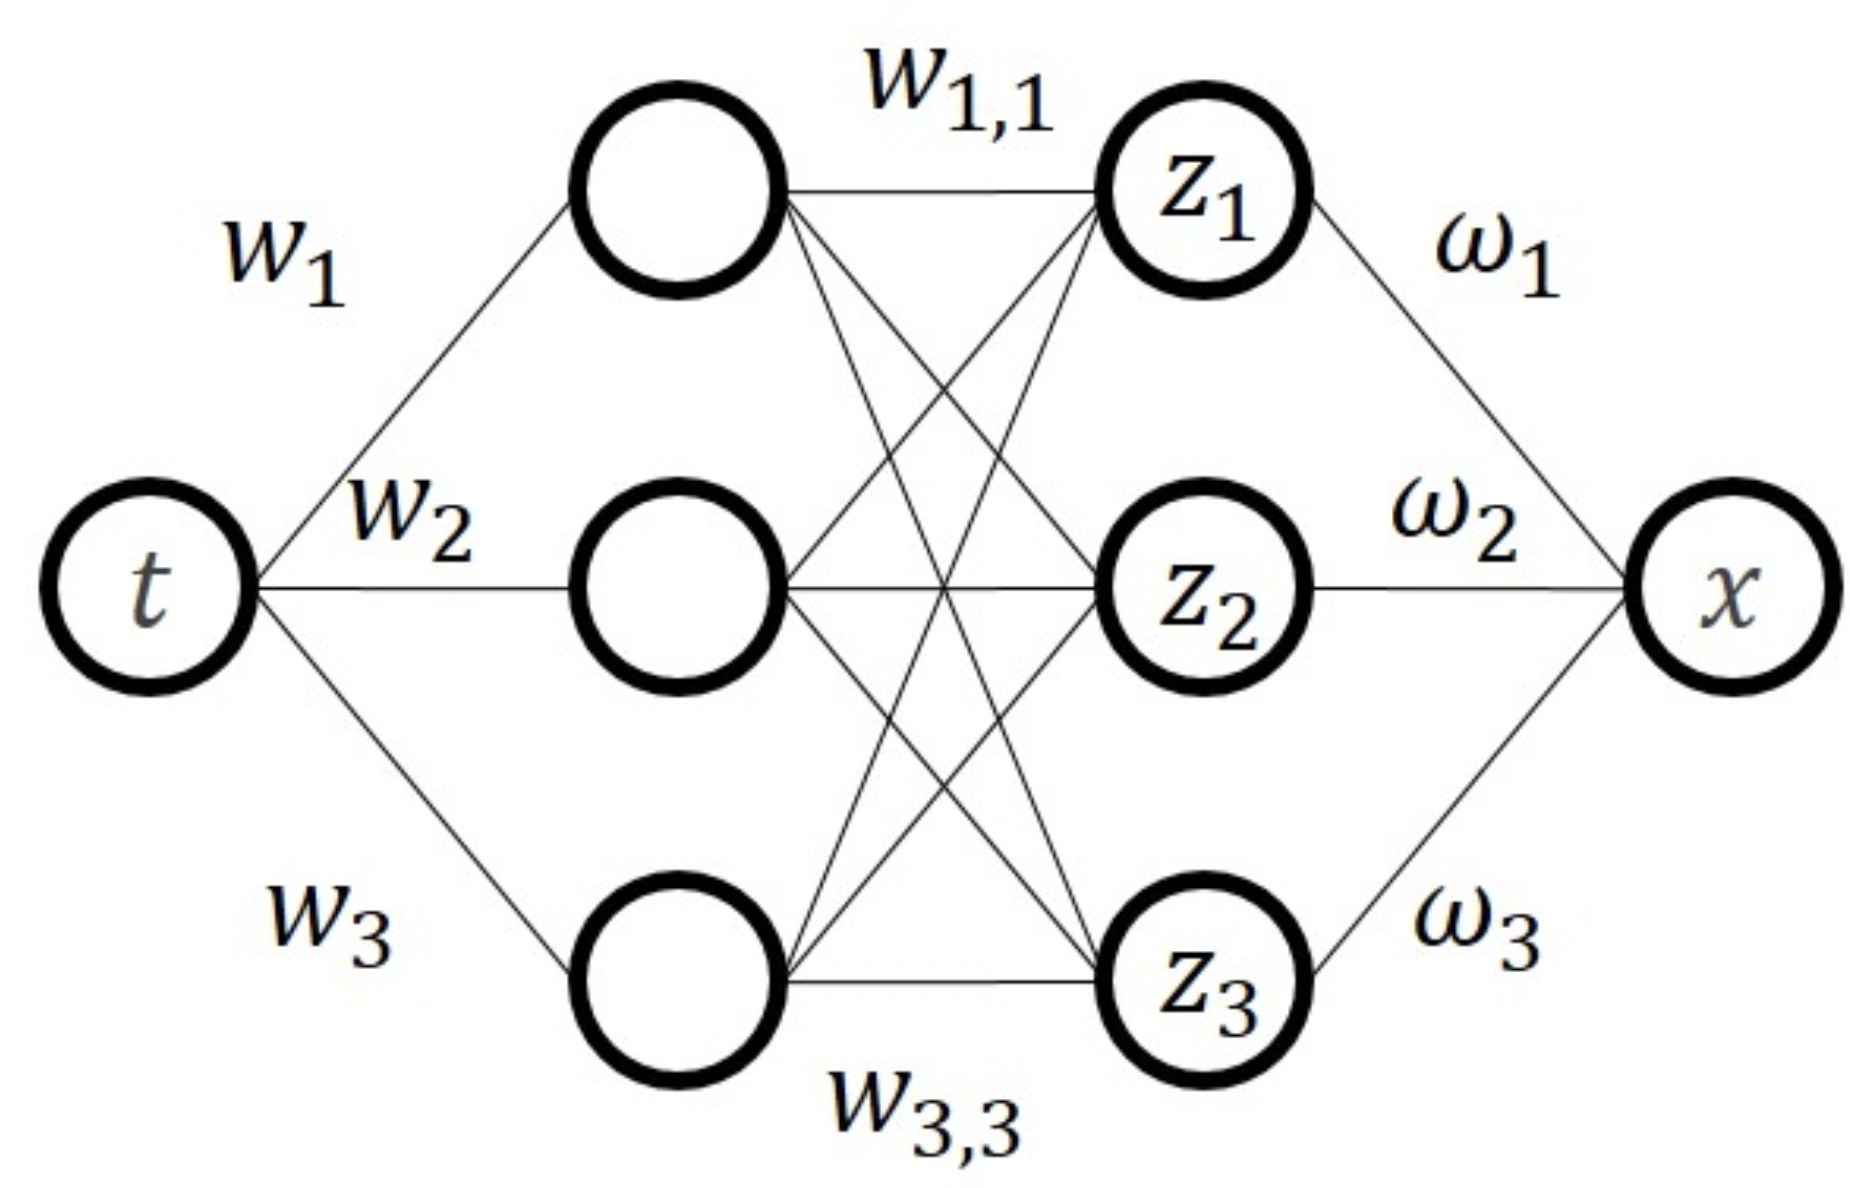
\includegraphics[width=\linewidth]{figure/fig1.png}
    \end{textblock*}
    \begin{textblock*}{0.4\linewidth}(230pt, 180pt)
      $L=\sum_{i}||x(t^i)-x_i||$
    \end{textblock*}
    Neural Network解
    \begin{align*}
      x(t)&=\omega_1z_1+\omega_2z_2+\omega_3z_3\\
      z_k(t)&=h(w_{1,k}h(w_1t)+w_{2,k}h(w_2t)w_{3,k}h(w_3t))
    \end{align*}
  学習データが必要, 学習データの範囲内でのみ性能保証.
  \end{enumerate}
\end{frame}

\begin{frame}
  % \frametitle{研究背景}    
  \setcounter{enumi}{3}
  \begin{enumerate}
    \item \alert{Physics Informed Neural Networks (PINNs)}\footfullcite{RAISSI2019686}\footfullcite{raissi_PhysicsinformedNeuralNetworks_2019}
  \end{enumerate}
 学習データの内容にとらわれずにNeural Networksを構築することはできないか?\\
 Neural Networks構築の上で学習データが大きく必要となる点は何か?\\
  $\rightarrow$ 損失関数\\
  \vspace{5pt}
  \structure{損失関数を学習データを用いず, 対象の方程式に沿った形で定義してやることができれば, 自然と対象の方程式の性質を孕んだNeural Networksが構成できる.}

  \begin{block}{背景}
    - 万能近似原理により, 深層学習が任意の関数を近似できる.\\
    - 自動微分により, 出力変数の入力変数に対する全ての微分項が得られる.
  \end{block}
  

\end{frame}

% \section{Physics Informed Neural Networks (PINNs)}
% \begin{frame}
%   \frametitle{Physics Informed Neural Networks (PINN)}

%   \begin{itemize}
%     \item 学習データを準備せずにNeural Networksを構築可能. 
%     \item 学習データに依存しない.
%     \item 対象となるモデルの微分方程式から損失関数を構成するため, 学習精度が高い. 
%     \item データ駆動的な手法を含むため, 新しい数理の発見の可能性を持っている. 
%   \end{itemize}  
%   損失関数に対象の現象(方程式)がもつ性質(境界条件, 初期条件)を用いて定義する. 
% \end{frame}

\begin{frame}
  \frametitle{PINNsの解決可能問題}
  \begin{itemize}
    \item 微分方程式の求解\\
    微分方程式の初期条件及び境界条件を損失関数に用いることで偏微分方程式の解を求める. 
    \item 微分方程式のパラメータ探索\\
    データをモデルとなる方程式に代入し, それと予測値の差から損失関数を構成し, パラメータを求める. 
  \end{itemize}
\end{frame}

\section{PINNsによる偏微分方程式の求解} 
\begin{frame}
  \frametitle{PINNsによる物理量の求解}
  % \vspace{3pt}
  非線形微分方程式
  \begin{align*}
    &u_{t}+\mathcal{N}[u;\lambda]=0, x \in \Omega, t \in[0, T]\\
    &\scriptsize \text{$u(t,x)$: 潜在解(latent (hidden) solution)}, 
    \text{$\mathcal{N}[\cdot;\lambda]$: 非線形項}, \text{$\omega \subset \mathbb{R}^D$}\normalsize
  \end{align*}
  Chain-ruleにおいて自動微分を用いてNetworksを構築する.\\
  \footnotesize $\rightarrow $微分演算子$\mathcal{N}$の作用により活性化関数は異なるが、通常$u(x,t)$を表現するNetworkと同じだけのパラメータを持つ。\normalsize
\end{frame}


\begin{frame}
  非線形微分方程式
  \begin{align*}
    f:=u_{t}+\mathcal{N}[u]=0,\quad  x \in \Omega, t \in[0, T]
  \end{align*}
  最小にすべき平均2乗誤差: \alert{$\mathrm{MSE}=\mathrm{MSE}_u+\mathrm{MSE}_f$}
  \begin{align*}
      &\alert{\mathrm{MSE}_{u}=\frac{1}{N_{u}} \sum_{i=1}^{N_{u}}\left|u\left(t_{u}^{i}, x_{u}^{i}\right)-u^{i}\right|^{2}}\quad \scriptsize\structure{\text{初期条件及び境界条件との差を評価}}\normalsize\\
      &\alert{\mathrm{MSE}_{f}=\frac{1}{N_{f}} \sum_{i=1}^{N_{f}}\left|f\left(t_{f}^{i}, x_{f}^{i}\right)\right|^{2}}\quad \scriptsize\structure{\text{f(x)を評価}}\normalsize
  \end{align*} 
  \scriptsize
  例: 自由落下問題
  \begin{align*}
    MSE=\underbrace{||x(0)-x_0||+\left|\left|\dfrac{\mathrm{d}x(0)}{\mathrm{d}t}-v_0\right|\right|}_{\text{初期条件との損失評価}}+\underbrace{\sum_{i}\left|\left|m\dfrac{\mathrm{d}^2x(t^i)}{\mathrm{d}t^2}-mg\right|\right|}_{\text{微分方程式との損失評価}}
  \end{align*}
  \normalsize
\end{frame}

\subsection{Example}
\begin{frame}
  \structure{例: (1次元非線形Schr\"{o}dinger方程式)}
  \begin{align*}
    f:=i\psi_t+\dfrac{1}{2}\psi_{xx}+|\psi|^2\psi=0, \quad x\in [-5,5], t\in [0,\pi/2]
  \end{align*}\vspace{-20pt}
  \scriptsize
  \begin{align*}
    \psi(0,x)=2\operatorname{sech}(x): \text{初期条件},\quad \psi(t,-5)=\psi(t,5), \psi_x(t,-5)=\psi_x(t,5)\text{周期境界条件}&\\
    (t: \text{時間}, x: \text{位置}, h: \text{複素数解})&
  \end{align*}
  \normalsize
  最小にすべき平均2乗誤差: \alert{$\mathrm{MSE}=\mathrm{MSE}_u+\mathrm{MSE}_f$}
  \footnotesize
  \begin{align*}
      &\alert{M S E_{u}=\frac{1}{N} \sum_{i=1}^{N}\left|u\left(t_{u}^{i}, x_{u}^{i}\right)-u^{i}\right|^{2}}\quad \structure{\text{: 予測値の平均2乗誤差}} \\
      &\alert{M S E_{f}=\frac{1}{N} \sum_{i=1}^{N}\left|f\left(t_{u}^{i}, x_{u}^{i}\right)\right|^{2}}\quad \structure{\text{: 微分方程式の平均2乗誤差}}\\
      &\alert{\mathrm{MSE}=|\hat{u}-u|^{2}+\left|\hat{u}_{t}+\lambda_{1} \hat{u} \hat{u}_{x}-\lambda_{2} \hat{u}_{x x}\right|^{2}}
  \end{align*}
  \vspace{-15pt}
  \normalsize
  \footnotesize
  \structure{なお, $\psi$は複素数であるが, $\psi=u+iv$としてそれぞれにNeural Networksを構成すればよい.}
  \normalsize
\end{frame}

\begin{frame}
  \begin{itemize}
    \item 計算結果
    \begin{figure}[H]
      \centering
        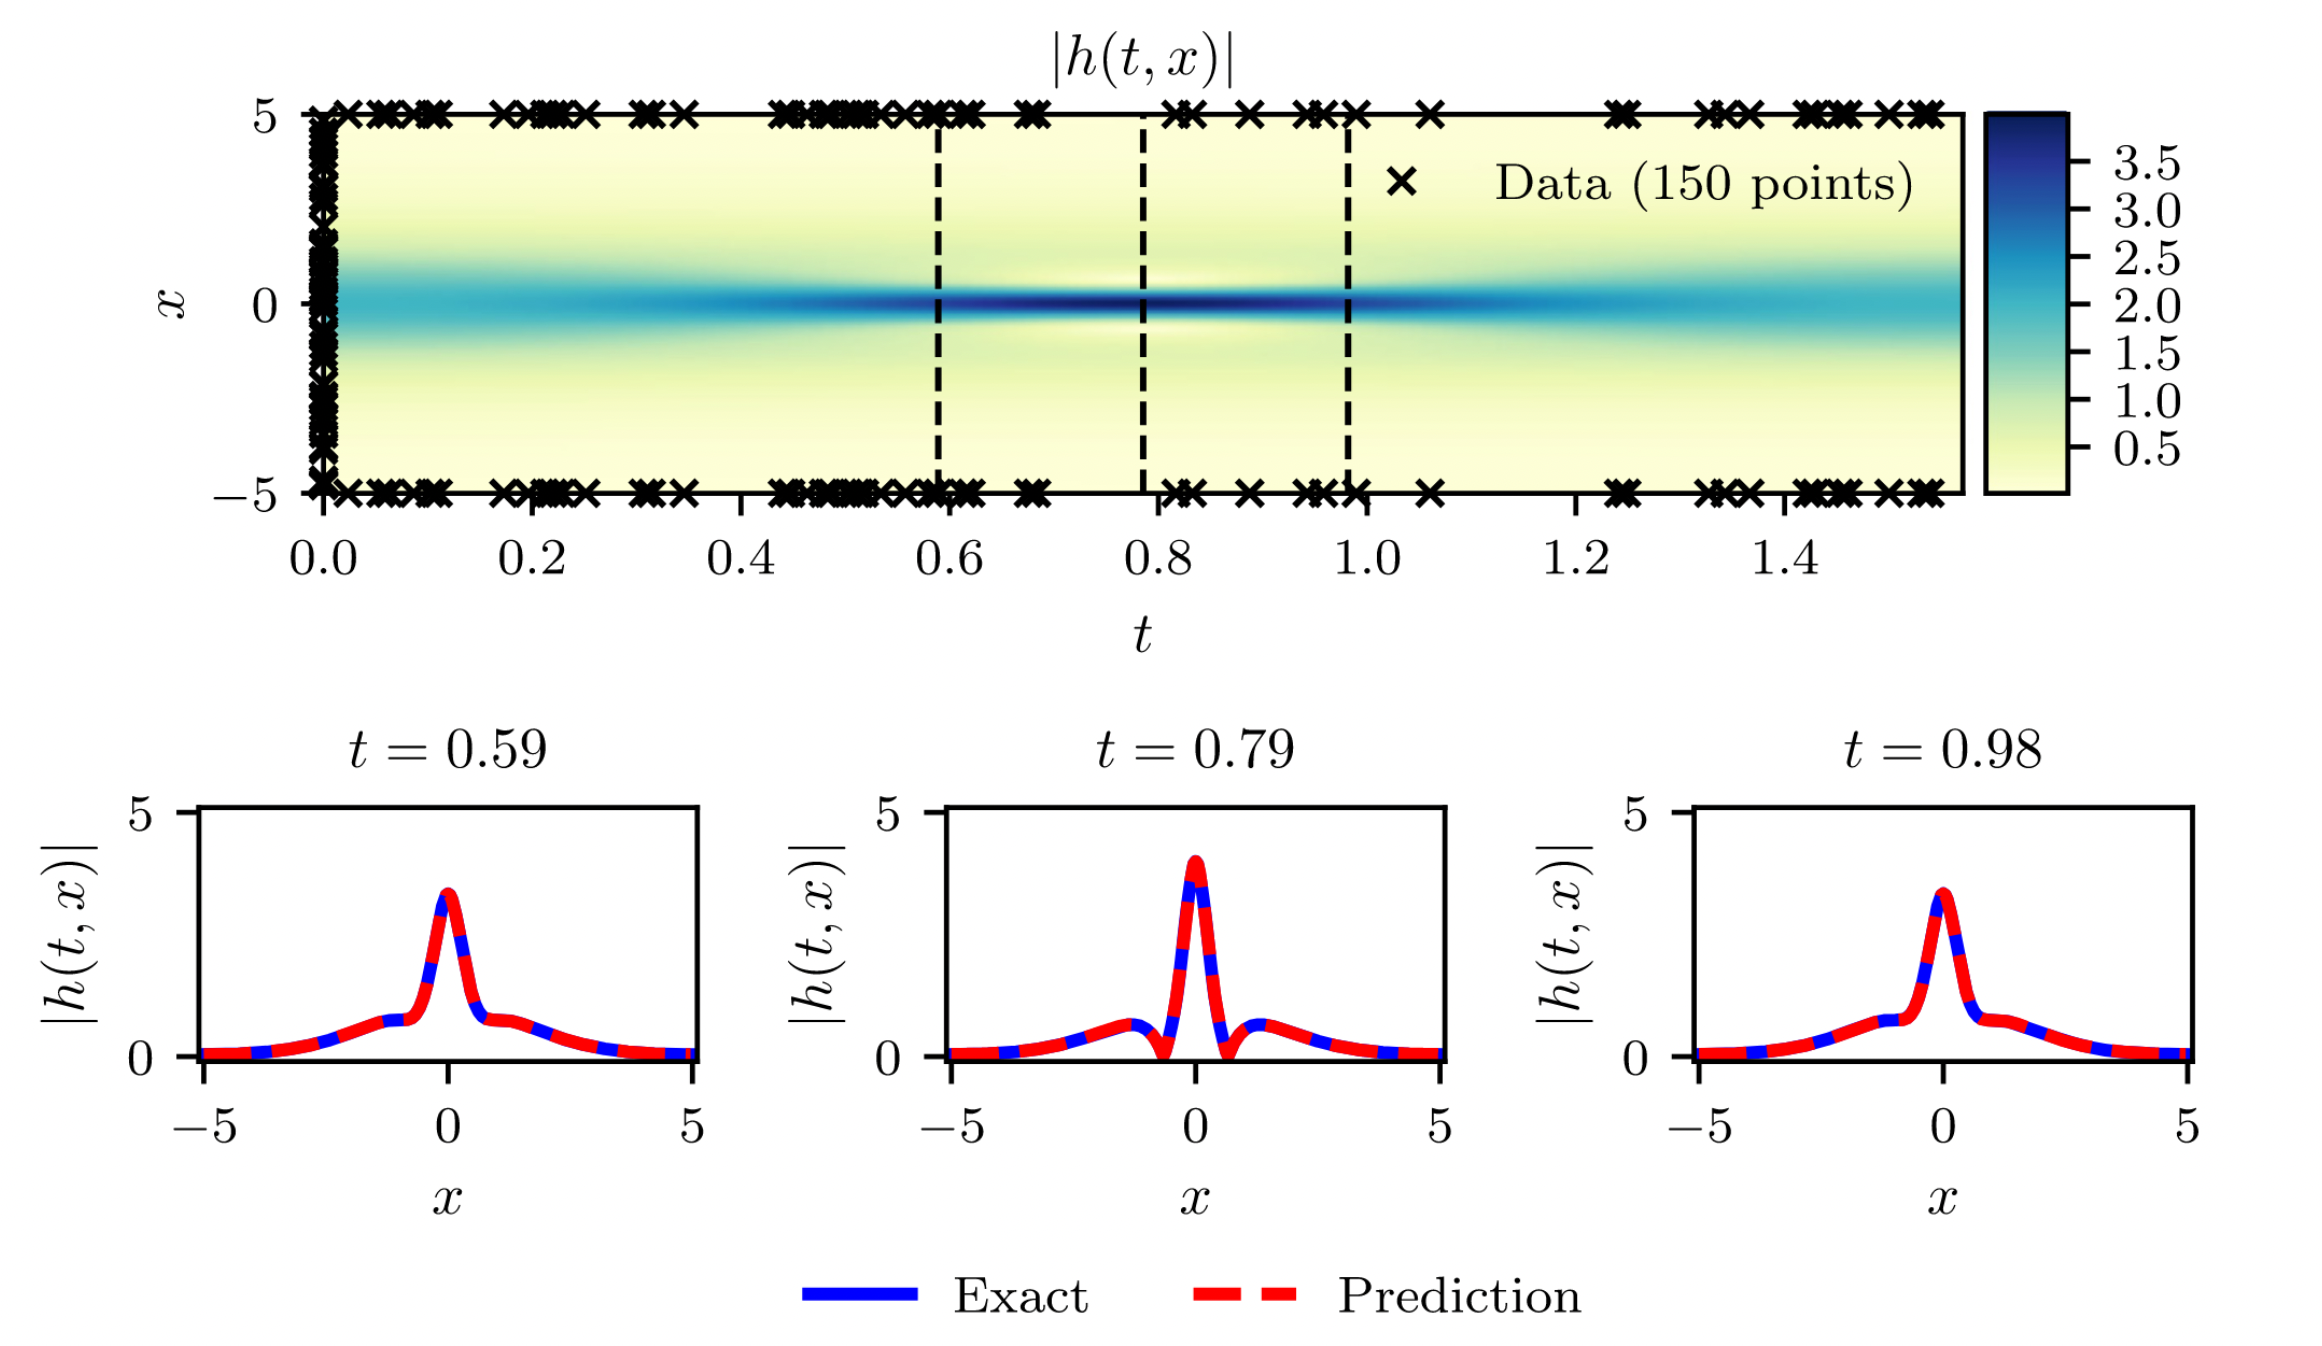
\includegraphics[width=0.9\linewidth]{figure/fig3.png}
    \end{figure}
    \tiny
    Data: 150 points, $N_b$: 50, $N_f$: 20000, 5-layer, 100 neurons
    \normalsize
  \end{itemize}
  \scriptsize
    厳密なシミュレーションと比較して, その精度の高さを確認($\mathrm{error}=1.97\times10^3$)
    \normalsize
\end{frame}
\begin{frame}
  \begin{itemize}
  \item 利点
  \begin{itemize}
    \item 訓練データはランダムな初期データを与えただけ.
    \item 少ないデータ量(150点)で再現可能.
  \end{itemize}
  \item 問題点
  \begin{itemize}
    \item 方程式に対する訓練データ$N_f$の多さ. 系の次元が増えるにつれ, 指数関数的に増加する.\\
    $\longrightarrow$ \quad 時間発展に関するRunge-Kutta法, Sparse Grid, quasi-Monte-Carlo samplingにより解決
  \end{itemize}
  \end{itemize}
\end{frame}

\section{PINNsによる微分方程式パラメータ探索}
\subsection{Example}
\begin{frame}
  \frametitle{PINNsによる微分方程式パラメータ探索}
既に対象となるモデルがサンプリングできていて, かつそれが従う方程式がわかっている場合のパラメーター推定を行う.
\vspace{3pt}
  例: Burgers方程式
  \begin{align*}
    f:=u_t+\lambda_1-\lambda_2u_{xx}=0
  \end{align*}
  \scriptsize
  学習データ: 既知のBurgers方程式の厳密解の描像における, 適当なデータ点
  \normalsize
  \begin{figure}[H]
    \centering
      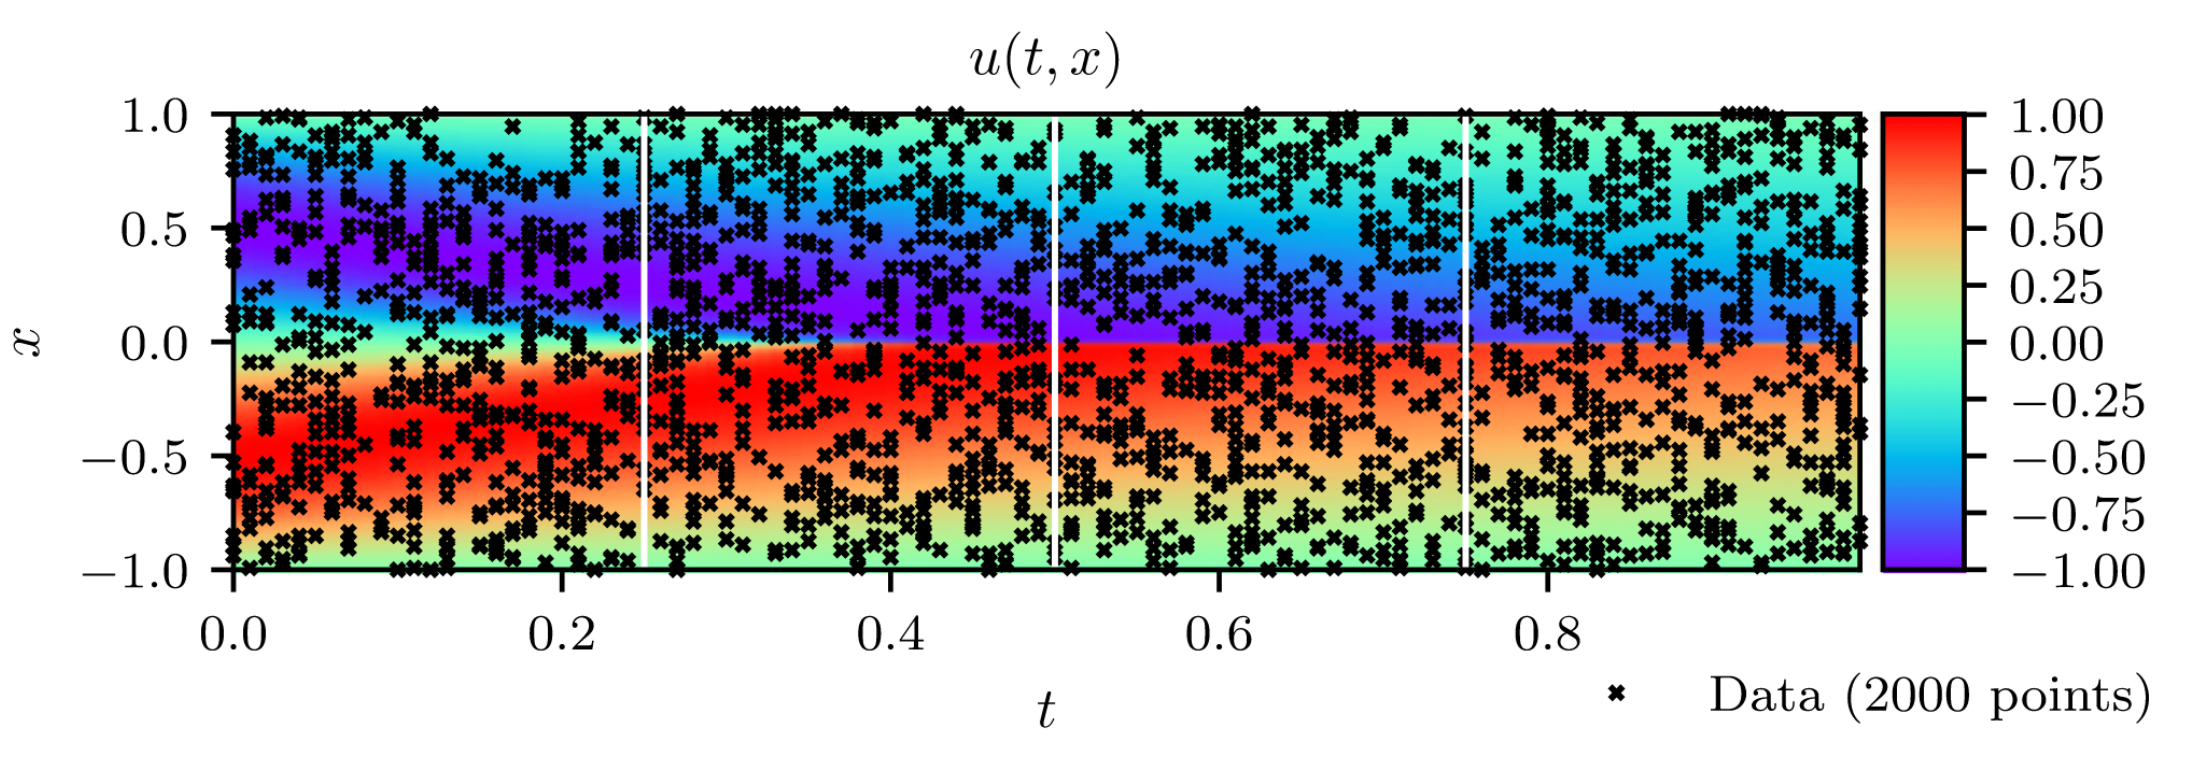
\includegraphics[width=0.8\linewidth]{figure/fig4.png}
  \end{figure}
\end{frame}

\begin{frame}
  最小にすべき平均2乗誤差: \alert{$\mathrm{MSE}=\mathrm{MSE}_u+\mathrm{MSE}_f$}
  \footnotesize
  \begin{align*}
      &\alert{M S E_{u}=\frac{1}{N} \sum_{i=1}^{N}\left|u\left(t_{u}^{i}, x_{u}^{i}\right)-u^{i}\right|^{2}}\quad \structure{\text{: 予測値の平均2乗誤差}} \\
      &\alert{M S E_{f}=\frac{1}{N} \sum_{i=1}^{N}\left|f\left(t_{u}^{i}, x_{u}^{i}\right)\right|^{2}}\quad \structure{\text{: 微分方程式の平均2乗誤差}}
  \end{align*}
  \normalsize
  \begin{itemize}
    \item 計算結果
    \begin{figure}[H]
      \centering
        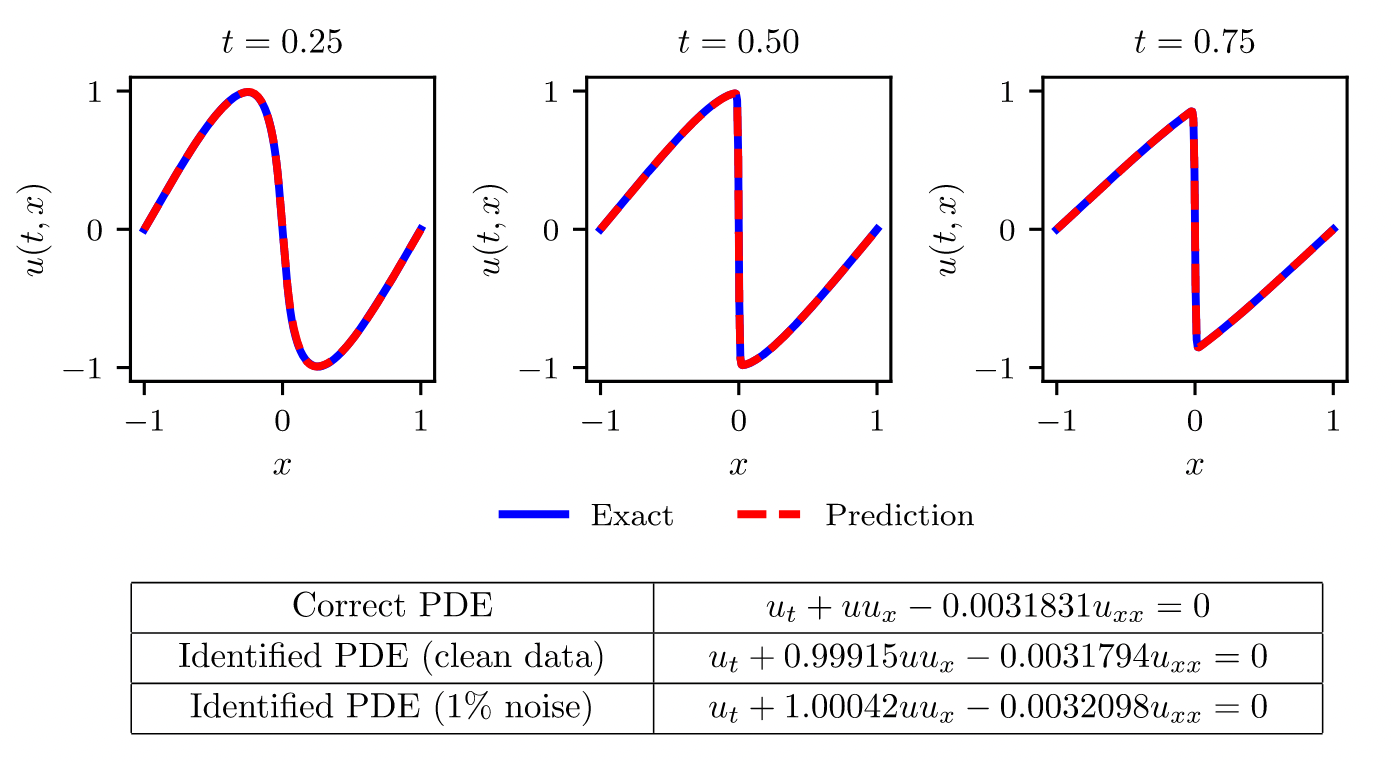
\includegraphics[width=0.7\linewidth]{figure/fig5.png}
    \end{figure}
  \end{itemize}
\end{frame}

\section{PINNsの利点と問題点}
\begin{frame}
  \frametitle{PINNsの利点と問題点}
  \frametitle{PINNの利点と問題点}
  \begin{itemize}
    \item 利点
    \begin{itemize}
      \item 損失関数の中に物理的要請を取り込むため, 学習データがランダム数でよい. 
      \item 学習データに依存しないため, 開発後の汎用性が高い. 
      \item 離散誤差を含むシミュレーション的手法より精度が高い.
    \end{itemize}
    \item 問題点
    \begin{itemize}
      \item 物理的要請(初期条件, 境界条件)を損失関数として用いるため, そららが変わる場合, 再学習する必要がある.\\
      $\rightarrow$\quad 境界条件が途中で変わる系とかキツい
      \item 損失関数の定義にどこまで物理的要請を組み込めば良いかわからない.
      \item 一応, 教師あり学習に当たるため, 事前に正解となるデータを蓄えておく必要がある.
    \end{itemize}
  \end{itemize}
\end{frame}

\section{今後個人的にすること}
\begin{frame}
  \frametitle{今後個人的にすること}
  hgoehoge
\end{frame}

\section{Appendix}
\subsection{計算フロー}
\begin{frame}
  \frametitle{計算フロー}
  \begin{tikzpicture}
  \tikzset{Process/.style={rectangle,  draw,  text centered, text width=3cm, minimum height=1cm}};
  \tikzset{Process2/.style={rectangle,  draw,  text centered, text width=4cm, minimum height=1cm}};
  \tikzset{Process3/.style={rectangle,  draw,  text centered, text width=4cm, minimum height=1cm}};
  \tikzset{Decision/.style={diamond,  draw,  text centered, aspect=3,text width=4cm, minimum height=0.5cm}};
  \node[Process] (a) {\scriptsize 1. ランダムでweightとバイアスを入力\normalsize};
  \node[Process][below=0.5cm of a] (b) {\scriptsize 2. 初期条件と境界条件の$(t_i,x_i)$を入力};
  \node[Process][below=0.5cm of b] (c) {\scriptsize 3. 予測値$\hat{u}$の出力};
  \node[Process][below=0.5cm of c] (d) {\scriptsize 4. 選点$(x_f,x_f)$における自動微分を計算};
  \node[Process2][right=3.5cm of b] (e) {\scriptsize 6. $w_{i+1}=w_i+\alpha\dfrac{\partial(\mathrm{MSE})}{\partial \bm{w}}$};
  \node[Decision][below=0.5cm of e] (f) {\scriptsize 5. $\mathrm{MSE}_u+\mathrm{MSE}_f<\mathrm{error}$};
  \node[Process][below=0.5cm of f] (g) {\scriptsize 7. 演算終了};
  \draw[->] (a) -- (b);
  \draw[->] (b) -- (c);
  \draw[->] (c) -- (d);
  \draw[->] (e) -- (b);
  \draw[->] (c) -- (d);
  \draw[->] (f) -- (e);
  \draw[->] (c) -- (f);
  \draw[->] (d) -- (f);
  \draw[->] (f) -- (g);
\end{tikzpicture}
\end{frame}

\subsection{自動微分}
\begin{frame}
    \frametitle{自動微分}
    プログラムによって定義された数学的な関数が与えられた時に, その導関数をアルゴリズムによって機械的に求める. 
  例: $f(a,b)=ab+\sin b$の導関数を機械的に計算するcite[hoge]. 
  \begin{flalign*}
    &\begin{aligned}
      &f=w+u\\
    &w=ab\\
    &u=\sin b
    \end{aligned}\quad
    \begin{aligned}
      \longrightarrow 
    \end{aligned}\quad
    \begin{aligned}
      &u'=\cos b\cdot b'\\
      &w'=a'b+ab'\\
      &f'=w'+u'
    \end{aligned}\quad
    \begin{aligned}
      \longrightarrow 
    \end{aligned}\quad
    \begin{aligned}
      &a'=\dfrac{\partial a}{\partial a}=1\\
      &b'=\dfrac{\partial b}{\partial b}=0\\
      &w'=\cos b \cdot b'\\
      &f'=w'+u'=b
    \end{aligned}&
  \end{flalign*}
  Chain-ruleを繰り返し利用することで偏導関数値を少ない計算量で自動的に求めることができる. (ライブラリが豊富)
\end{frame}





\begin{frame}[allowframebreaks]{参考文献}
  \printbibliography
\end{frame}



% \frame{\centering \Large Thank you for your attention !!}


\end{document}